\chapter{Desarrollo en Robotstudio}\label{chp-06}

La idea principal del proyecto es orientar el sistema para la realización de prácticas de 
laboratorio, por lo que el trabajo a realizar por los alumnos está en la programación en 
Robotstudio. Por esta razón, este capítulo va orientado a dar las pautas necesarias para el 
funcionamiento del sistema y su integración en el ecosistema de ABB.

\section{Funcionamiento sin microcontrolador}

El caso más simple de funcionamiento es cuando no hay microcontrolador. En este caso se
utilizarán las entradas y salidas digitales del controlador para realizar los movimientos.
La conexión entre las salidas digitales de la caja y el controlador se realiza mediante 
un módulo de interfaz como el mostrado en la figura \ref{fig:interfazfisicadigital}.

\begin{figure}[hbtp]
    \centering
    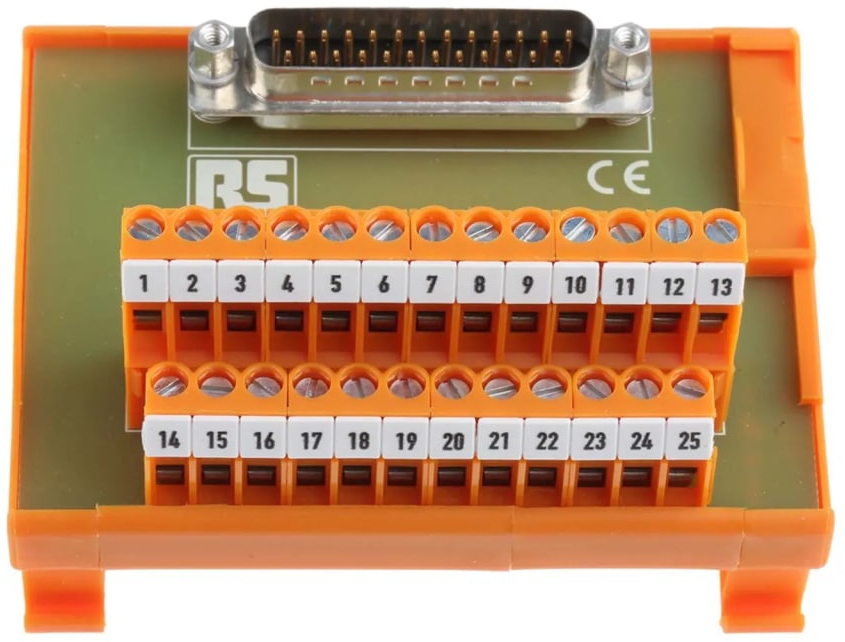
\includegraphics[width=\textwidth/2]{06-robotstudio/interfazdigital.jpg}
    \caption{Amplificación señales calibre digital a 5V}
    \label{fig:interfazfisicadigital}
    \end{figure}

Dicho módulo se conecta a la placa DSQC 652 que se encuentra montada en el controlador del robot.
Este dispositivo está diseñado para manejar señales digitales entre el sistema del robot y sistemas
como el de este proyecto. Los pines expuestos en el módulo de interfaz son los siguientes:
\begin{itemize}
    \item Entradas (DI, Digital Inputs). Pines del 1 al 8 que corresponden a los DI01 a DI08.
    \item Salidas (DO, Digital Outputs). Pines del 14 al 24 que corresponden a los DO01 a DO08.
    \item GND. Pin 24.
    \item VCC 24V. Pin 25.
\end{itemize}

En el los pines de salida se conectarán las señales de Avance y Retroceso, mientras que en los
de entrada estarán la señal del sensor fotoeléctrico, la emergencia, el estado de la señal local y
la señal micro.

Las funciones referentes a las señales digitales se pueden consultar en el manual de RAPID \cite{rapid}.
Las más relevantes para el uso básico son:
\begin{itemize}
    \item SetDO, cambio de valor en salida digital. Uso: SetDo señalDO, valor;
    \item Lectura de entrada digital. Se puede realizar simpelmente utilizando el nombre de la señal. 
    Usos: estado-actual := señalDI; IF señalDI = valor DO ...
    \item WaitDI, espera en el programa hasta que una señal de entrada tome cierto valor.
    Uso: WaitDI señalDI, valor;
\end{itemize}

Un ejemplo de programa es el que se puede ver en \ref{no_micro}. Este programa consiste en hacer avanzar
la cinta hasta que se enciende el sensor fotoeléctrico, que el robot recoja la pieza y repita la operación
haciéndolo retroceder. Para ello, se debe definir el \textit{workobject} de la cinta transportadora para mover
el brazo robótico sobre sus ejes. Posteriormenete se debe definir la posición de recogida del brazo donde 
se activa el sensor fotoeléctrico. Las demás posiciones se generarán mediante offsets de la posición de recogida.
El trabajo con el brazo robótico queda a cargo de futuros alumnos, aquí se muestra exclusivamente el trato 
con las señales digitales. Para simplificar los nombres de las señales se utilizan nombres descriptivos, no
el que realmente aparece en RobotStudio.

\begin{lstlisting}[language=,caption={Ejemplo de programa sin microcontrolador}, breaklines=true, label=no_micro]
MODULE Module1
    !Aquí deben estar definidas las posiciones y variables auxiliares
    !
    PROC main()
        !Se procede a avanzar 
        SetDO señalAvance, 1;
        SetDO señalRetroceso, 0;

        !Se espera a que se active el sensor fotoeléctrico
        WaitDI señalFoto, 1;
        !Se para la cinta
        SetDO señalAvance, 0;
        SetDO señalRetroceso, 0;
        
        !Movimiento del brazo robótico para recoger la pieza y colocarla en una posición avanzada donde haya que retroceder
        ...

        !Misma operación a la inversa
        SetDO señalAvance, 0;
        SetDO señalRetroceso, 1;

        !Se espera a que se active el sensor fotoeléctrico
        WaitDI señalFoto, 1;
        !Se para la cinta
        SetDO señalAvance, 0;
        SetDO señalRetroceso, 0;

        !Movimiento del brazo robótico para recoger la pieza y colocarla en la posición original
        ...
    ENDPROC
END MODULE
\end{lstlisting}

\section{Funcionamiento con microcontrolador}